\documentclass[12pt]{article}
\usepackage[english]{babel}
\usepackage[utf8x]{inputenc}
\usepackage{amsmath}
\usepackage{graphicx}
\usepackage[font=small,labelfont=bf]{caption}
\usepackage[colorinlistoftodos]{todonotes}
\usepackage{csquotes}
\usepackage[official]{eurosym}
\usepackage{fancyhdr}
\usepackage[a4paper,bindingoffset=0.2in,%
            left=1in,right=1in,top=1in,bottom=1in,%
            footskip=.25in]{geometry}
\usepackage{blindtext}

\newgeometry{left=0.8in,right=0.8in,top=1in,bottom=1in}
\pagestyle {fancy}
\fancyhf{}
\rhead{Midterm Report - Manalath}
\lhead{\leftmark}
\rfoot{\thepage}

\begin{document}
\begin{titlepage}

\newcommand{\HRule}{\rule{\linewidth}{0.25mm}} % Defines a new command for the horizontal lines, change thickness here

\center % Center everything on the page

%----------------------------------------------------------------------------------------
%	HEADING SECTIONS
%----------------------------------------------------------------------------------------

\textsc{\LARGE Faculdade de Engenharia da Universidade do Porto}\\[0.5cm] % Name of your university/college
\textsc{\Large Mestrado Integrado em Engenharia Informática e Computação}\\[0.5cm] % Major heading such as course name
\textsc{\large Logic Programming}\\[0.5cm] % Minor heading such as course title

%----------------------------------------------------------------------------------------
%	TITLE SECTION
%----------------------------------------------------------------------------------------

\HRule \\[0.75cm]
{ \huge \bfseries Manalath}\\[0.4cm] % Title of your document
\HRule \\[1cm]

%----------------------------------------------------------------------------------------
%	AUTHOR SECTION
%----------------------------------------------------------------------------------------

\begin{minipage}{0.6\textwidth}
\begin{flushleft} \large
\emph{Autores:}\\
Bruno Vale \textsc{Fernandes}\\
Tiago \textsc{Magalhães}\\

\end{flushleft}
\end{minipage}
~
\begin{minipage}{0.35\textwidth}
\begin{flushright} \large
\emph{Supervisor:} \\
Dr. Daniel \textsc{Silva} % Supervisor's Name
\end{flushright}
\end{minipage}\\[1cm]

%----------------------------------------------------------------------------------------
%	LOGO SECTION
%----------------------------------------------------------------------------------------

\includegraphics[width=50mm,scale=0.5]{feuplogo.png}\\[0.5cm] % FEUP Logo



% If you don't want a supervisor, uncomment the two lines below and remove the section above
%\Large \emph{Author:}\\
%John \textsc{Smith}\\[3cm] % Your name

%----------------------------------------------------------------------------------------
%	DATE SECTION
%----------------------------------------------------------------------------------------

{\large October 2018}\\[2cm] % Date, change the \today to a set date if you want to be precise

%----------------------------------------------------------------------------------------

\vfill % Fill the rest of the page with whitespace

\end{titlepage}
\tableofcontents
\pagebreak

\section{History}
  \hspace{0.6cm}
  Manalath is a an abstract game for two players from the family of Yavalath-like
  games, however unlike Yavalath, Manalath was designed by humans.

  The game was created in 2012 by  Dieter Stein and Néstor Romeral Andrés.

  The name Manalath comes from the latin \textit{'manus'}, referring to the five
  fingers of the human hand.

  Like Yavalath the game is played on a hexgonal board and the win condition depends on the number of pieces of the same color in a row.
\subsection{Yavalath-like Games}
\hspace{0.6cm}
  Yavalath was a game created in 2007, where players play in a hexagonal board and win by being able to put 4 pieces of their color in a row and
  lose if they put 3 pieces in a row.
  However distinguishing it from regular games Yavalath has a particularity. It
  was designed, developed and tested by a computer through the use of genetic
  algorithms.

  The computer program that created Yavalath, named \textbf{Ludi} takes the rules
  of existing games and scrambles them together using genetic algorithms and
  assigning a score to the created game based on how interesting to a human the
  game is believed to be. The entire testing and evaluation process is automated
  which allowed Ludi to create 1389 games in the span of 4 week's, 19 of which
  were deemed to be interesting to humans.

  Over time the idea of making games like Yavalath that were designed by a
  computer became popular. Manalath is one of the offspring's of this game design
  fashion, however unlike many of its siblings it was designed by a humans and
  not by computers.

\pagebreak
\section{Rules}
\hspace{0.6cm}
    In this section we will be presenting the rules for the game Manalath, this is
    the Components that make up the game, the rules for piece movement, the conditions
    in which a game ends and variants of the game.
  \subsection{Components}
\hspace{0.6cm}
    A Manalath game has the following pieces/components:
    \begin{itemize}
        \item A 5-5-6 Hexagonal board with 70 spaces.
        \item 25 Orange game pieces.
        \item 25 Purple game pieces.
  \end{itemize}
\subsection{Piece Movement}
\hspace{0.6cm}
  The game board begins empty with the game pieces next to the board
  in reaching distance to the players.

  Each of the players has one unique color, either orange or purple. The orange
  player starts the game.

  Each turn the player puts one of the pieces on an empty space on the board, players can
  place any piece that has not yet been placed, this includes a piece of the opposing
  color, the only restrictions present is that the placement of a piece may never
  form a group of more than 5 pieces of the same color.
\subsection{Game End Condition}
\hspace{0.6cm}
  There are 3 distinct ways to end a game of Manalath, these are verified
  at the end of the players turn:
  \begin{enumerate}
    \item When there are 5 pieces of the current players color in a group, the player wins the game
    \item When there are 4 pieces of the current players color in a group, the player loses the game
    \item When there are no longer any possible legal moves, the game ends in a tie.
  \end{enumerate}

A losing condition takes precedence over a winning conditions,
so in case you have both the winning and losing condition at the end of your turn
you lose the game.
\subsection{Variant}
\hspace{0.6cm}
There is one optional variant to the game. There exist 3 green pieces that can
be places anywhere on the board before the beginning of the game.

The two players must agree on how many of these pieces to use and where to place
them.

This variant tends to make the games shorter but richer as the pieces act as
unplayable spaces.

\pagebreak
\section{Representation}

\hspace{0.6cm}
We will now proceed to explain out internal representation for the game board
and we intend to develop it, the we will explain out initial textural representation,
how we implemented it and how we print it.
\subsection{Internal Representation}
\hspace{0.6cm}
Our internal representation is currently a simple list based representation. We
have a list with several lists for each row of out board, these lists then contain
the value of the cells of the board.

The elements of the list have 4 different possible values to allows us to
represent the board:
\begin{itemize}
  \item A -1 represents a white space used for board indentation.
  \item A 1 represents an empty cell of the board.
  \item A 2 represents an X on the cell of the board or rather a purple piece.
  \item A 3 represents an O on the cell of the board or rather an orange piece.
\end{itemize}

Later on we intend on creating predicates that help us identify specific cells of
the board according to our cell labeling scheme.

We are labeling our cells in a diagonal form going from a to j, in a bottom to left
diagonal, then we can label the cells in each diagonal from 0 to 8 in the largest
diagonal. This allows us to numerically execute permutations on adjacent cells
which then will help us check for groups of pieces.

\subsection{Text Based Representation}
\hspace{0.6cm}
As previously explained we have a list of lists, we will now explain the predicates
we created to print the board.

First of all we have the predicate symbol(number, Variable), this predicate acts as
a dictionary or hash tables that maps the numbers in the lists to their correct textural
representation, this is done by giving to Variable the value of the character. The
way we did this was by creating multiples instances of this predicate where the value
of number was already filled in acting as several disjunctions that would translate to the sentence
 $$(-1 \Rightarrow ` \ `)  \vee (1 \Rightarrow `\#`) \vee (2 \Rightarrow `X`)
\vee (3 \Rightarrow `O`) $$

Next we have the predicate printLine([H $|$ T]), this predicates print a list that corresponds
to a line of the board, to do this it splits the head of the list from the rest
of the list, then it passes the value of the head to the symbol predicate to extract
the correct representation, it then prints that character and recursively calls
itself (printLine) for the rest of the list to be printed.

Finally we have the predicate printBoard([H $|$ T]), this predicate prints the whole
board, to do this is separates the first list from the rest of the lists. It then
call the predicate printLine for the first list and call itself recursively for
the rest of the lists.

You can see below images of this board representation in various games states.

\begin{center}
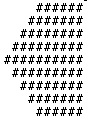
\includegraphics[width=0.3\linewidth]{start_game_print.png} % Game Print
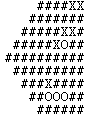
\includegraphics[width=0.3\linewidth]{mid_game_print.png} % Game Print
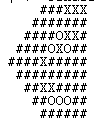
\includegraphics[width=0.3\linewidth]{game_print.png} % Game Print
\captionof{figure}{Game representation in an start of game state,mid of game state
and end of game state, respectively}
\end{center}

\end{document}
